```
\subsection{Coaxial Magic: The Antenna Matching Wonder!}

\begin{tcolorbox}[colback=gray!10, colframe=black, title=E9E02]
What antenna matching system matches coaxial cable to an antenna by connecting the shield to the center of the antenna and the conductor a fraction of a wavelength to one side?

\begin{enumerate}[label=\Alph*.]
    \item \textbf{Gamma match}
    \item Delta match
    \item T-match
    \item Stub match
\end{enumerate} \end{tcolorbox}

\subsubsection{Elaboration on Related Concepts}

Antenna matching systems are vital in radio communication because they ensure maximum power transfer between the transmission line (coaxial cable) and the antenna. The gamma match is a specific type of antenna matching system that utilizes a $\gamma$ (gamma) configuration to match the impedance between the coaxial cable and the antenna effectively. 

In the gamma match setup, the outer conductor or shield of the coaxial cable is connected to the center of the antenna. The inner conductor is then connected to a point on the antenna that is one-quarter wavelength away from the gamma connection point. This configuration allows the antenna to be tuned effectively for resonance, which minimizes standing wave ratios (SWR) and maximizes the radiated power.

The importance of matching lies in the fact that when the impedance of the antenna system is not matched to the transmission line, reflections can occur, leading to losses and reduced efficiency in the transmission of the radio signal.

\subsubsection{Calculation and Diagram}

If we were to calculate a specific frequency for the setup, we would base our calculations on the wavelength, $\lambda$, which is related to the frequency, $f$, and the speed of light, $c$:

\[
\lambda = \frac{c}{f}
\]

For example, if we want to match a system to a frequency of 144 MHz (a common frequency in amateur radio), we would use:

\[
c \approx 3 \times 10^8 \text{ m/s}
\]
\[
\lambda = \frac{3 \times 10^8 \text{ m/s}}{144 \times 10^6 \text{ Hz}} \approx 2.0833 \text{ m}
\]

Now, determining the point for the gamma connection, we set it at a quarter wavelength, which would be:

\[
\frac{\lambda}{4} = \frac{2.0833 \text{ m}}{4} \approx 0.5208 \text{ m}
\]

This distance is critical for effective tuning of the antenna.

To illustrate the gamma matching system, we can draw a simple diagram using TiKZ:

\begin{center}
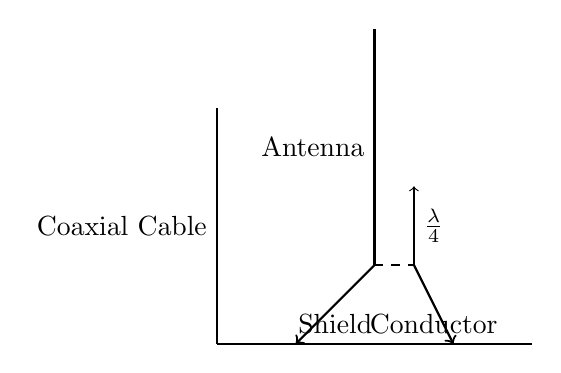
\begin{tikzpicture}
    % Draw the antenna
    \draw[thick] (0,0) -- (0,3) node[midway,left] {Antenna} ;
    
    % Draw the coaxial cable
    \draw[thick] (-2,-1) -- (2,-1);
    \draw[thick] (-2,-1) -- (-2,2) node[midway,left] {Coaxial Cable};
    
    % Draw the connections
    \draw[->, thick] (0,0) -- (-1,-1) node[midway,below] {Shield};
    \draw[->, thick] (0.5,0) -- (1,-1) node[midway,below] {Conductor};
    
    % Mark the quarter wavelength
    \draw[dashed] (0,0) -- (0.5,0);
    \draw[->] (0.5,0) -- (0.5,1) node[midway,right] {$\frac{\lambda}{4}$};
    
    % Draw the ground
    \draw[dashed] (-2,-1) -- (2,-1);
\end{tikzpicture}
\end{center}
```